\documentclass[aspectratio=169,12pt]{beamer}

% Compila com pdflatex/lualatex/xelatex padrão, sem pacotes exóticos.
\usetheme{default}
\usecolortheme{whale}

\usepackage[utf8]{inputenc}
\usepackage[T1]{fontenc}
\usepackage[brazil]{babel}
\usepackage{graphicx}
\usepackage{booktabs}
\usepackage{amsmath}
\usepackage{xcolor}
\usepackage{tikz}
\usetikzlibrary{arrows.meta,positioning}

\graphicspath{{figures/}{../results/LDM_Conditional_Attributes/}}

% ---- paleta ------------------------------------------------------------
% amber  = método adotado / final
% teal   = explorado, não escolhido
% cinza  = dados / infraestrutura
\definecolor{ink}{HTML}{1D2024}
\definecolor{amber}{HTML}{A8591B}
\definecolor{ambersoft}{HTML}{F1E3D2}
\definecolor{teal}{HTML}{3F6B66}
\definecolor{tealsoft}{HTML}{E6EDEC}
\definecolor{graysoft}{HTML}{EEECE2}
\definecolor{inkdim}{HTML}{55585E}

\setbeamercolor{palette primary}{bg=ink,fg=white}
\setbeamercolor{palette secondary}{bg=ink,fg=white}
\setbeamercolor{palette tertiary}{bg=ink,fg=white}
\setbeamercolor{title}{fg=ink}
\setbeamercolor{frametitle}{bg=ink,fg=white}
\setbeamercolor{structure}{fg=amber}
\setbeamercolor{block title}{bg=ambersoft,fg=amber}
\setbeamercolor{block body}{bg=graysoft,fg=ink}
\setbeamertemplate{navigation symbols}{}
\setbeamertemplate{itemize item}{\color{amber}$\bullet$}
\setbeamerfont{frametitle}{series=\bfseries}

% ---- rótulo de status no canto (eyebrow) --------------------------------
\newcommand{\statuslabel}[2]{%
  \begin{tikzpicture}[remember picture, overlay]
    \node[anchor=north east, xshift=-0.4cm, yshift=-0.35cm,
          fill=#1, text=white, rounded corners=2pt,
          inner sep=3pt, font=\scriptsize\bfseries] at (current page.north east) {#2};
  \end{tikzpicture}%
}
\newcommand{\statusfinal}{\statuslabel{amber}{MÉTODO FINAL}}
\newcommand{\statusexplorado}{\statuslabel{teal}{NÃO ESCOLHIDO}}
\newcommand{\statusdados}{\statuslabel{inkdim}{DADOS}}

\title{Difusão Latente Condicional para Edição de Atributos Faciais\\ com Preservação de Identidade}
\author{Lucas Barcelos}
\institute{Machine Learning 2 --- IMPA}
\date{}

\begin{document}

% ---------------------------------------------------------------- título
\begin{frame}[plain]
  \titlepage
\end{frame}

% ------------------------------------------------------------ o problema
\begin{frame}{O problema}
  Dada uma foto de uma pessoa:
  \begin{itemize}
    \item extrair a \textbf{identidade} (quem é)
    \item ler os \textbf{atributos faciais} (CelebA, 40 binários: sorriso, óculos, cor de cabelo, \dots)
    \item o usuário escolhe quais atributos mudar
    \item gerar uma nova imagem: \textbf{mesma identidade, atributos editados}
  \end{itemize}
  \vspace{0.3cm}
  Duas condições que precisam conviver sem uma vazar na outra.

  \vspace{0.3cm}
  {\small\color{inkdim}\emph{Modelo de base: \textit{latent diffusion model} --- treinado para
  reverter um processo de ruído gaussiano no espaço latente de um VAE.
  (revisão rápida, não vou reexplicar difusão)}}

  \note{Abrir dizendo o que o projeto faz em uma frase: ``dado uma foto, editar
  atributos faciais preservando a identidade da pessoa''. Essa é a única
  menção a ``o que é difusão'' do talk inteiro --- uma frase, sem fórmula de
  forward/reverse process. Plateia já conhece. O ponto central do slide é a
  tensão identidade vs.\ atributo, que motiva o resto da apresentação.}
\end{frame}

% ------------------------------------------------------- pipeline (visão)
\begin{frame}{Pipeline de dados --- visão geral}
  \statusdados
  CelebA: 202.599 imagens, já alinhadas numa convenção \textbf{nunca
  publicada} oficialmente.

  \vspace{0.2cm}
  Por imagem, temos:
  \begin{itemize}
    \item 40 atributos binários (\texttt{list\_attr\_celeba.csv})
    \item identidade da pessoa --- múltiplas fotos por identidade (\texttt{identity\_CelebA.txt})
    \item 5 landmarks faciais (\texttt{list\_landmarks\_align\_celeba.csv})
  \end{itemize}

  \vspace{0.2cm}
  Nenhum script de treino de difusão lê imagem crua: tudo passa por caches
  pré-computados. {\small\color{inkdim}(detalhes mais adiante)}

  \note{Rápido --- é só inventário do dataset. Os caches ganham slide próprio
  depois.}
\end{frame}

% --------------------------------------------------------- pseudo-arq
\begin{frame}{Pseudo-arquitetura}
  \begin{center}
  \resizebox{\textwidth}{!}{%
  \begin{tikzpicture}[
      box/.style={draw=inkdim, rounded corners=2pt, minimum height=0.8cm, align=center, font=\scriptsize},
      arr/.style={-{Stealth[length=2mm]}, draw=inkdim}
    ]
    \node[box, minimum width=2.6cm] (img) {foto};
    \node[box, minimum width=2.6cm, right=1.0cm of img] (vae) {VAE.encode};
    \node[box, minimum width=2.6cm, right=1.0cm of vae] (z) {latente $z$};

    \node[box, minimum width=3.2cm, below=0.7cm of img] (ref) {foto de referência};
    \node[box, minimum width=3.2cm, right=0.6cm of ref] (idenc) {encoder de identidade};
    \node[box, minimum width=2.8cm, right=0.6cm of idenc] (idtok) {tokens de id};

    \node[box, minimum width=3.2cm, below=0.55cm of ref] (attr) {atributos desejados};
    \node[box, minimum width=3.2cm, right=0.6cm of attr] (attrenc) {embedder de atributos};
    \node[box, minimum width=2.8cm, right=0.6cm of attrenc] (attrtok) {tokens de atributo};

    \node[box, fill=amber!12, draw=amber, minimum width=2.6cm, below right=0.7cm and 2.6cm of z] (cond) {condicionamento};
    \node[box, fill=amber!12, draw=amber, minimum width=2.2cm, right=0.6cm of cond] (unet) {U-Net};
    \node[box, minimum width=2.2cm, right=0.6cm of unet] (zp) {$z'$};
    \node[box, minimum width=2.6cm, below=0.55cm of unet] (dec) {VAE.decode};
    \node[box, minimum width=2.8cm, below=0.55cm of zp] (out) {imagem editada};

    \draw[arr] (img) -- (vae);
    \draw[arr] (vae) -- (z);
    \draw[arr] (ref) -- (idenc);
    \draw[arr] (idenc) -- (idtok);
    \draw[arr] (attr) -- (attrenc);
    \draw[arr] (attrenc) -- (attrtok);
    \draw[arr] (z.south) |- (cond.west);
    \draw[arr] (idtok.south) |- (cond.west);
    \draw[arr] (attrtok.north) |- (cond.west);
    \draw[arr] (cond) -- (unet);
    \draw[arr] (unet) -- (zp);
    \draw[arr] (zp) -- (out);
    \draw[arr] (unet) -- (dec);
    \draw[arr] (dec) -- (out);
  \end{tikzpicture}%
  }
  \end{center}

  \vspace{0.15cm}
  {\small Por enquanto, \textbf{condicionamento} e \textbf{U-Net} são
  caixas-pretas --- o foco agora é só entender que existem duas condições
  entrando por um mecanismo comum.}

  \note{Não abrir a U-Net nem o cross-attention aqui. Isso vem depois,
  quando comparar CFG/CG.}
\end{frame}

% --------------------------------------------------------- CFG vs CG
\begin{frame}{Como condicionar duas coisas ao mesmo tempo?}
  \statusexplorado
  \begin{center}
  \small
  \begin{tabular}{@{}p{2.8cm}p{7.2cm}@{}}
    \toprule
    \textbf{Mecanismo} & \textbf{Como funciona} \\
    \midrule
    CFG \newline {\scriptsize Classifier-Free Guidance} &
      dropout do condicionante no treino; na inferência, interpola
      $\epsilon_{uncond}$ / $\epsilon_{cond}$ \\[0.3cm]
    CG \newline {\scriptsize Classifier Guidance} &
      classificador externo sobre o latente ruidoso $z_t$; usa
      $\nabla \log p(y\mid z_t)$ para empurrar a amostra \\
    \bottomrule
  \end{tabular}
  \end{center}

  \vspace{0.25cm}
  Ideia original do projeto: \textbf{CFG para identidade + CG para
  atributos}, simultaneamente (``Mixed Guidance'').

  \vspace{0.15cm}
  {\small Na prática, o CG dos atributos teve três problemas estruturais:}
  \begin{itemize}\small
    \item \textbf{sigmoid satura} --- classificador confiante $\Rightarrow$ gradiente colapsa
    \item $\log p(y\mid z_t)$ soma os \textbf{40 atributos} --- os 39 que não mudam dominam o gradiente do único que se quer editar
    \item classificador no latente: $t$ alto $\approx$ ruído puro (aprende só o prior), $t$ baixo funciona mas sobram poucos passos para editar
  \end{itemize}

  \note{Esse é o motivo histórico de Ho \& Salimans (2022) proporem CFG ---
  comparação eps vs.\ eps não satura e escala estável. Passar rápido pelos 3
  motivos, eles justificam a mudança de método no próximo slide.}
\end{frame}

% --------------------------------------------------------- composable cfg
\begin{frame}{Solução: Composable CFG \small(Liu et al., ECCV 2022)}
  \statusfinal
  Identidade e atributos viram \textbf{dois condicionantes independentes} ---
  três forward passes da U-Net por passo de amostragem:

  \begin{block}{}
  \centering
  \begin{equation*}
    \epsilon = \epsilon(\varnothing,\varnothing)
      + s_{id}\big[\epsilon(id,\varnothing) - \epsilon(\varnothing,\varnothing)\big]
      + s_{attr}\big[\epsilon(id,attr) - \epsilon(id,\varnothing)\big]
  \end{equation*}
  \end{block}

  \begin{itemize}\small
    \item $s_{id}$ --- o quanto a identidade puxa a geração
    \item $s_{attr}$ --- o quanto os atributos deslocam, \textbf{dado} que a
      identidade já foi aplicada (por isso o segundo termo usa
      $\epsilon(id,\varnothing)$ como base, não $\epsilon(\varnothing,\varnothing)$)
  \end{itemize}

  \vspace{0.15cm}
  {\small Cada escala é ajustável de forma independente --- sem o problema de
  saturação do CG, porque o sinal é sempre uma diferença de $\epsilon$'s.}

  \vspace{0.15cm}
  {\small No treino, cada amostra do batch sorteia independentemente entre 4
  combinações de dropout (id only / attr only / ambos / nenhum) --- o modelo
  precisa aprender as 4 distribuições marginais que a fórmula usa na
  inferência.}

  \note{Uma das duas ideias centrais do talk. Enfatizar: o segundo termo usa
  $\epsilon(id,\varnothing)$, não $\epsilon(\varnothing,\varnothing)$ --- é
  isso que torna o termo de atributo ortogonal ao de identidade em vez de
  competir com ele.}
\end{frame}

% --------------------------------------------------------- não escolhidos
\begin{frame}{Métodos e arquiteturas não escolhidos}
  \statusexplorado
  Ordem aproximada de exploração:
  \begin{itemize}\small
    \item \texttt{train\_cond.py} --- só atributos, sem identidade
    \item \texttt{train\_image\_cond.py} --- identidade via encoder
      \emph{treinável} (ResNet-18 truncado) em vez de ArcFace congelado
    \item \texttt{train\_mixed\_guidance*.py} --- CFG (identidade) + CG
      (atributos) juntos, o ``Mixed Guidance'' original do objetivo do projeto
  \end{itemize}

  \vspace{0.2cm}
  {\small Resultado do estágio só-atributos (\texttt{train\_cond.py}, época
  450, sem condicionamento de identidade):}

  \begin{center}
    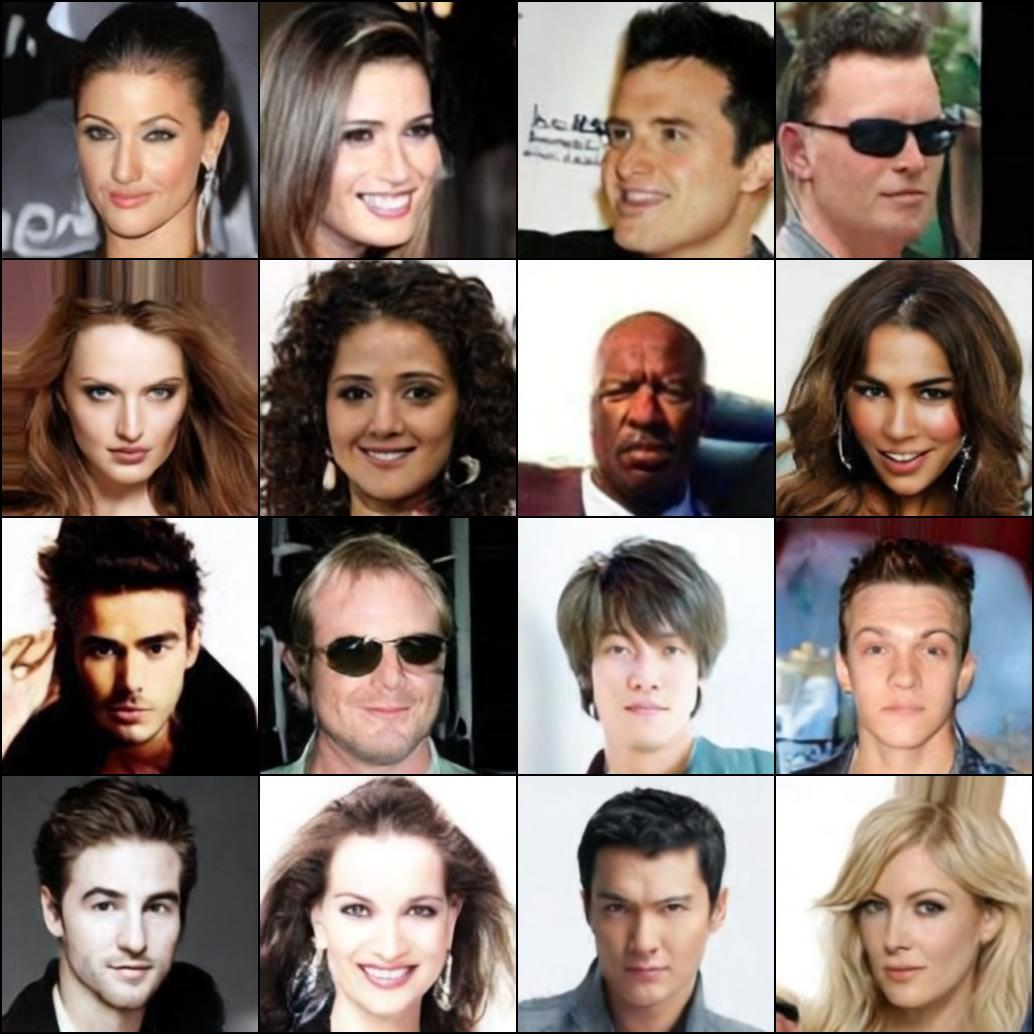
\includegraphics[height=3.6cm]{450.jpg}
  \end{center}

  \note{Essas são rodadas anteriores reais, não o método final. Deixar claro
  que essas imagens NÃO usam identidade --- servem para mostrar que a U-Net
  aprende os atributos, mas ainda faltava a parte de identidade + o Mixed
  Guidance esbarrou nos 3 problemas do CG do slide anterior.}
\end{frame}

% --------------------------------------------------------- método final
\begin{frame}{Composable CFG com referência pareada}
  \statusfinal
  {\small \texttt{train/train\_cfg\_composable\_paired.py} + \texttt{generate\_cfg\_composable.py}}

  \vspace{0.2cm}
  {\small Mesma fórmula de 3 termos do slide anterior, com uma correção importante:}

  \begin{block}{}
  \small A foto usada pelo encoder de identidade é uma foto
  \textbf{diferente} da mesma pessoa (via \texttt{identity\_CelebA.txt}) ---
  não a própria imagem-alvo do denoising.
  \end{block}

  {\small \textbf{Por que isso importa:} usando a mesma foto como alvo e como
  referência de identidade, os tokens de identidade (CLIP) vazavam a
  expressão exata do alvo --- $s_{attr}$ não conseguia mudar atributos
  ligados à expressão (ex.: \texttt{Smiling}), porque o ``sorriso'' já estava
  embutido na condição de identidade. Pareando com outra foto da mesma
  pessoa, a identidade fica desacoplada da expressão/pose daquela imagem
  específica.}

  \begin{itemize}\small
    \item Encoder: \texttt{clip\_arcface} (CLIP ViT-B/32 + ArcFace, 16 tokens) ou \texttt{arcface\_only}
    \item Atributos: \texttt{AttributeEmbedder} --- 40 tokens, um por atributo binário
    \item U-Net: sem modificação --- cross-attention já atende a todos os tokens concatenados
  \end{itemize}

  \note{Essa é a ideia mais importante do talk, junto com a fórmula de 3
  termos. Explicar o vazamento com uma frase concreta: ``se a foto de
  referência já está sorrindo, pedir smiling=0 na geração não adianta,
  porque o CLIP da própria referência já carrega o sorriso''.}
\end{frame}

% --------------------------------------------------------- resultados final
\begin{frame}{Resultados do método final}
  \statusfinal
  \begin{center}
  \begin{block}{}
    \small Treino em andamento --- ainda não há checkpoints/curvas do
    \texttt{train\_cfg\_composable\_paired.py} para mostrar aqui.

    \vspace{0.2cm}
    \emph{(placeholder --- inserir aqui print do TensorBoard e pares
    \texttt{<epoch>\_attr\_orig.jpg} / \texttt{<epoch>\_attr\_smile.jpg}
    quando disponíveis)}
  \end{block}
  \end{center}

  \note{Ser honesto sobre isso --- não inventar curva nem reaproveitar
  imagem de rodada antiga como se fosse o resultado final. Pode falar do
  critério de avaliação: comparar attr\_orig vs.\ attr\_smile na mesma
  época, julgando fidelidade visual vs.\ força da edição.}
\end{frame}

% --------------------------------------------------------- caches
\begin{frame}{Pipeline de dados em detalhe --- três caches}
  \statusdados
  {\small Nenhum script de treino de difusão lê imagem crua --- tudo passa
  por um destes caches pré-computados:}

  \vspace{0.15cm}
  \begin{center}
  \scriptsize
  \begin{tabular}{@{}p{2.3cm}p{4.2cm}p{2.6cm}@{}}
    \toprule
    \textbf{Cache} & \textbf{Conteúdo} & \textbf{Usado por} \\
    \midrule
    \texttt{cache\_latent/} & \texttt{latent[4,32,32]} (VAE, $\mu\cdot0.18215$, determinístico) + \texttt{attrs[40]} & treino de difusão \\
    \texttt{cache\_encoder/} & \texttt{arcface[512]} + \texttt{clip[seq\_len,768]} & encoder de identidade \\
    \texttt{cache\_aligned\_celeba/} & crop 224$\times$224 (template ArcFace) & classificador de atributos \\
    \bottomrule
  \end{tabular}
  \end{center}

  \vspace{0.2cm}
  {\small \texttt{cache\_latent} e \texttt{cache\_encoder} usam a
  \textbf{mesma} convenção de recorte (\texttt{CenterCrop(178)→Resize(256)},
  o crop nativo do CelebA). Só o cache do classificador usa um recorte
  diferente --- de propósito (próximo slide).}

  \note{Enfatizar a tabela --- é o slide de referência técnica caso alguém
  pergunte ``onde entra tal encoder''.}
\end{frame}

% --------------------------------------------------------- alinhamento
\begin{frame}{Alinhamento --- dois templates, dois propósitos}
  \statusdados
  {\small O algoritmo de alinhamento original do CelebA nunca foi publicado
  --- não existe um único ``alinhamento correto''.}
  \begin{itemize}\small
    \item \texttt{FaceAligner} (template ArcFace, saída 224$\times$224) ---
      usado só para treinar o classificador de atributos (CLIP ViT-L/14
      fine-tunado)
    \item \texttt{CelebAAligner} (template nativo do CelebA, derivado
      empiricamente da média dos 5 landmarks sobre as 202.599 imagens) ---
      saída 178$\times$218, compatível com o crop usado pelo VAE / encoder
      de identidade
  \end{itemize}

  {\small \textbf{Por quê dois:} VAE, ArcFace e o encoder de identidade
  foram treinados só sobre o crop nativo do CelebA. Alinhar uma selfie real
  com o template ArcFace e passar pro resto do pipeline geraria uma imagem
  fora da distribuição de treino, degradando identidade.}

  \begin{columns}
    \begin{column}{0.48\textwidth}
      \centering
      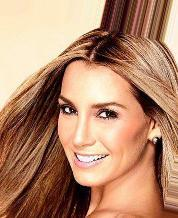
\includegraphics[height=2.6cm]{orig01.png}\\
      {\scriptsize original (crop nativo)}
    \end{column}
    \begin{column}{0.48\textwidth}
      \centering
      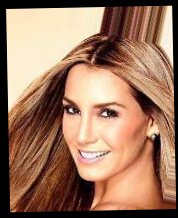
\includegraphics[height=2.6cm]{aligned01.png}\\
      {\scriptsize após CelebAAligner}
    \end{column}
  \end{columns}
  \vspace{0.1cm}
  {\scriptsize\color{inkdim}\emph{Diferença imperceptível --- confirma que o
  CelebAAligner preserva imagens já alinhadas.}}

  \note{Apontar que as duas imagens são quase idênticas --- esse é o ponto:
  alinhar algo que já está alinhado não deveria mudar nada.}
\end{frame}

% --------------------------------------------------------- validação simulada
\begin{frame}{Validação simulada do alinhamento}
  \statusdados
  {\small Para validar o \texttt{CelebAAligner} sem depender de fotos reais
  soltas, simulamos uma foto ``fora do padrão'': rotação + deslocamento
  sintéticos sobre uma imagem já alinhada do CelebA.}

  \begin{columns}
    \begin{column}{0.48\textwidth}
      \centering
      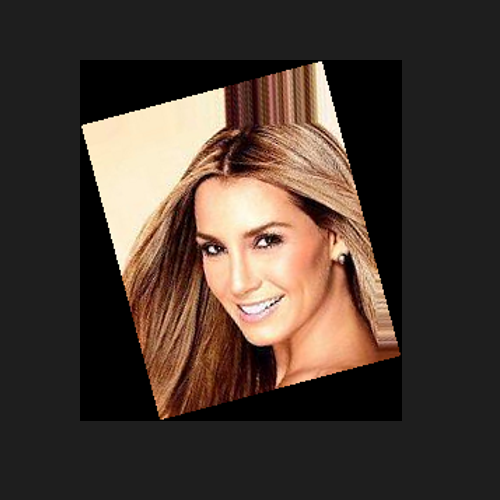
\includegraphics[height=2.8cm]{perturbed.png}\\
      {\scriptsize perturbada (sintético)}
    \end{column}
    \begin{column}{0.48\textwidth}
      \centering
      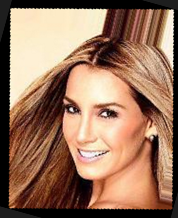
\includegraphics[height=2.8cm]{corrected.png}\\
      {\scriptsize corrigida via CelebAAligner}
    \end{column}
  \end{columns}

  \vspace{0.2cm}
  {\small \texttt{CelebAAligner} recupera o enquadramento nativo do CelebA a
  partir da perturbação. \textbf{Ainda não conectado} a nenhum script de
  geração --- hoje \texttt{generate\_from\_ref.py}/\texttt{generate\_cfg\_composable.py}
  só fazem \texttt{CenterCrop}+\texttt{Resize}, sem detecção de rosto.}

  \note{Essa é a validação ``de laboratório'' antes de testar com fotos
  reais soltas. Deixar claro que ainda é um gap conhecido, não algo já
  integrado.}
\end{frame}

% --------------------------------------------------------- próximos passos
\begin{frame}{Estado atual e próximos passos}
  \begin{itemize}
    \item Treinar \texttt{train\_cfg\_composable\_paired.py} até convergência
      e coletar resultados/TensorBoard reais
    \item Conectar \texttt{CelebAAligner} na entrada dos scripts de geração,
      para aceitar fotos arbitrárias (não só imagens já no formato CelebA)
    \item Trocar \texttt{AttributePredictor} (não treinado) por
      \texttt{CLIPAttributeClassifier} já treinado, para ler atributos de
      uma foto de referência real
    \item Ideias arquiteturais para depois de ter um baseline:
      cross-attention dual (estilo IP-Adapter) ou adaLN-Zero/FiLM para os
      atributos, em vez de concatenar tudo num único cross-attention
  \end{itemize}

  \note{Fechar com honestidade sobre o que falta --- mostra maturidade do
  projeto, não fraqueza.}
\end{frame}

% --------------------------------------------------------- obrigado
\begin{frame}[plain]
  \begin{center}
    \Huge Obrigado\\[0.4cm]
    \normalsize\color{inkdim} Perguntas?
  \end{center}
\end{frame}

\end{document}
